\documentclass[aspectratio=169]{beamer}
\usetheme{Madrid}
\usecolortheme{default}
\setbeamertemplate{navigation symbols}{}
\beamerdefaultoverlayspecification{<+->}

\usepackage[utf8]{inputenc}
\usepackage[T1]{fontenc}
\usepackage{lmodern}
\usepackage{amsmath,amssymb}
\usepackage{booktabs}
\usepackage{listings}
\usepackage{xcolor}
\usepackage{graphicx}
\usepackage{hyperref}

\title[AlphaStock in Indian Markets]{AlphaStock in Indian Stock Market\\From Paper Understanding to Full Implementation}
\author{Dhairya Kantawala}
\institute{IIT Bombay}
\date{\today}

\definecolor{codebg}{RGB}{248,248,248}
\definecolor{codekw}{RGB}{0,61,153}
\definecolor{codecm}{RGB}{0,120,0}
\definecolor{codestr}{RGB}{153,51,0}

\lstdefinestyle{mypython}{
  language=Python,
  backgroundcolor=\color{codebg},
  basicstyle=\ttfamily\scriptsize,
  keywordstyle=\color{codekw}\bfseries,
  commentstyle=\color{codecm},
  stringstyle=\color{codestr},
  showstringspaces=false,
  breaklines=true,
  frame=single,
  tabsize=2
}

\begin{document}

\begin{frame}
  \titlepage
\end{frame}

\begin{frame}{Roadmap}
  \tableofcontents
\end{frame}

\section{Transition from Proposal to Execution}
\begin{frame}{What the First Presentation Promised}
  \begin{itemize}
    \item Original plan: implement AlphaStock for NIFTY 500 universe.
    \item Pipeline commitment: Bloomberg data \textrightarrow{} cleaning \textrightarrow{} feature engineering \textrightarrow{} RL model.
    \item Extension idea: replace paper's LSTM encoder with simpler MLP to reduce overfitting risk.
    \item Target metric remained Sharpe ratio (risk-adjusted performance), not only raw returns.
  \end{itemize}
\end{frame}

\begin{frame}{What Was Actually Built}
  \begin{itemize}
    \item End-to-end data pipeline across \texttt{raw\_data}, \texttt{semi\_clean\_data}, \texttt{final\_clean\_data}, and \texttt{normalised\_data}.
    \item Reusable helper API in \texttt{helper\_functions.py} for consistent state/reward generation.
    \item Full implementation notebook: \texttt{alphastock\_mlp.ipynb}.
    \item Training, evaluation, and diagnostics plots exported for reporting.
  \end{itemize}
\end{frame}

\section{Data Pipeline for Indian Market}
\begin{frame}{Data Engineering Workflow}
  \begin{center}
  \large
  Bloomberg Export $\rightarrow$ Raw CSVs $\rightarrow$ Semi-cleaned Data\\
  $\rightarrow$ Final Clean Data $\rightarrow$ Normalized Features $\rightarrow$ RL States/Rewards
  \end{center}
  \vspace{0.4cm}
  \begin{itemize}
    \item Universe aligned to Indian equities (NSE/BSE tickers present in cleaned datasets).
    \item Monthly feature creation and rolling normalization to avoid leakage.
    \item Reward definition kept consistent with long-short AlphaStock formulation.
  \end{itemize}
\end{frame}

\begin{frame}[fragile]{Feature Engineering (Implemented)}
\begin{lstlisting}[style=mypython]
def get_normalised_data(file):
    df = pd.read_csv("final_clean_data/"+file, index_col=0)
    df['ret_1m'] = np.log(df['price'] / df['price'].shift(1))
    df['ret_3m'] = np.log(df['price'] / df['price'].shift(3))
    df['mom_12m'] = df['price'] / df['price'].shift(12) - 1
    df['vol_3m'] = df['ret_1m'].rolling(3).std()
    df['vol_6m'] = df['ret_1m'].rolling(6).std()
    # ... volume, valuation, size and composite factors ...
    rolling_mean = df[features].rolling(24).mean().shift(1)
    rolling_std  = df[features].rolling(24).std().shift(1)
    df[features] = (df[features] - rolling_mean) / (rolling_std + 1e-8)
    df['R'] = (df['price'].shift(-1) / df['price'])
\end{lstlisting}
\end{frame}

\begin{frame}[fragile]{State and Reward Interface}
\begin{lstlisting}[style=mypython]
def get_state_reward(time):
    month = months[time]
    state_i, reward_i = [], []
    for file in files_list:
        try:
            stock_data = pd.read_csv('normalised_data/'+file, index_col=0)
            s_i = stock_data.loc[month][features]
            r_i = stock_data.loc[month]['R']
            state_i.append(s_i)
            reward_i.append(r_i)
        except:
            continue
    return state_i, reward_i
\end{lstlisting}
\end{frame}

\section{Model and Training}
\begin{frame}[fragile]{Architecture Extension: MLP + Cross-Stock Attention}
\begin{lstlisting}[style=mypython]
class MLPEncoder(nn.Module):
    def __init__(self, input_dim, hidden_dim, output_dim, dropout=0.2):
        super().__init__()
        self.net = nn.Sequential(
            nn.Linear(input_dim, hidden_dim), nn.BatchNorm1d(hidden_dim),
            nn.ReLU(), nn.Dropout(dropout),
            nn.Linear(hidden_dim, hidden_dim), nn.BatchNorm1d(hidden_dim),
            nn.ReLU(), nn.Dropout(dropout),
            nn.Linear(hidden_dim, output_dim)
        )
\end{lstlisting}
\begin{itemize}
  \item Original AlphaStock idea preserved: learn stock representations then model cross-asset dependencies.
  \item Practical change: LSTM replaced with compact MLP encoder.
\end{itemize}
\end{frame}

\begin{frame}[fragile]{Cross-Asset Attention (Core AlphaStock Mechanism)}
\begin{lstlisting}[style=mypython]
class CrossStockAttention(nn.Module):
    def forward(self, r):
        Q = self.WQ(r); K = self.WK(r); V = self.WV(r)
        scores = torch.matmul(Q, K.T) / math.sqrt(self.d_model)
        alpha = F.softmax(scores, dim=1)
        A = torch.matmul(alpha, V)
        s = self.ws(A).squeeze(-1)
        return s
\end{lstlisting}
\begin{itemize}
  \item Winner score for each stock is conditioned on all other stocks.
  \item Enables relative ranking needed for long-short portfolio construction.
\end{itemize}
\end{frame}

\begin{frame}[fragile]{Sharpe-Oriented Loss}
\begin{lstlisting}[style=mypython]
def compute_loss(R_list, H0=0.0):
    R = torch.stack(R_list)
    mu = R.mean()
    sigma = R.std() + 1e-6
    sharpe = mu / sigma
    cumulative = torch.cumprod(1 + R, dim=0)
    peak = torch.cummax(cumulative, dim=0).values
    drawdown = ((peak - cumulative) / (peak + 1e-8)).max()
    loss = -0.5 * (sharpe - H0) - 0.5 * mu * 12 + 0.2 * drawdown
    return loss
\end{lstlisting}
\begin{itemize}
  \item Maintains paper objective while adding practical drawdown regularization.
\end{itemize}
\end{frame}

\begin{frame}{Training Snapshot}
  \begin{itemize}
    \item Parameters: 3,025 trainable.
    \item Input dimension: 14 engineered features.
    \item Sliding-window trajectory training on precomputed monthly states.
    \item Holdout setup: last 24 months used for testing.
  \end{itemize}
  \vspace{0.2cm}
  \begin{block}{Observed Training Behavior}
    Epoch Sharpe moved from \textasciitilde0.48 to \textasciitilde1.78 with stable learning-rate schedule.
  \end{block}
\end{frame}

\begin{frame}{Training Curves}
  \begin{center}
    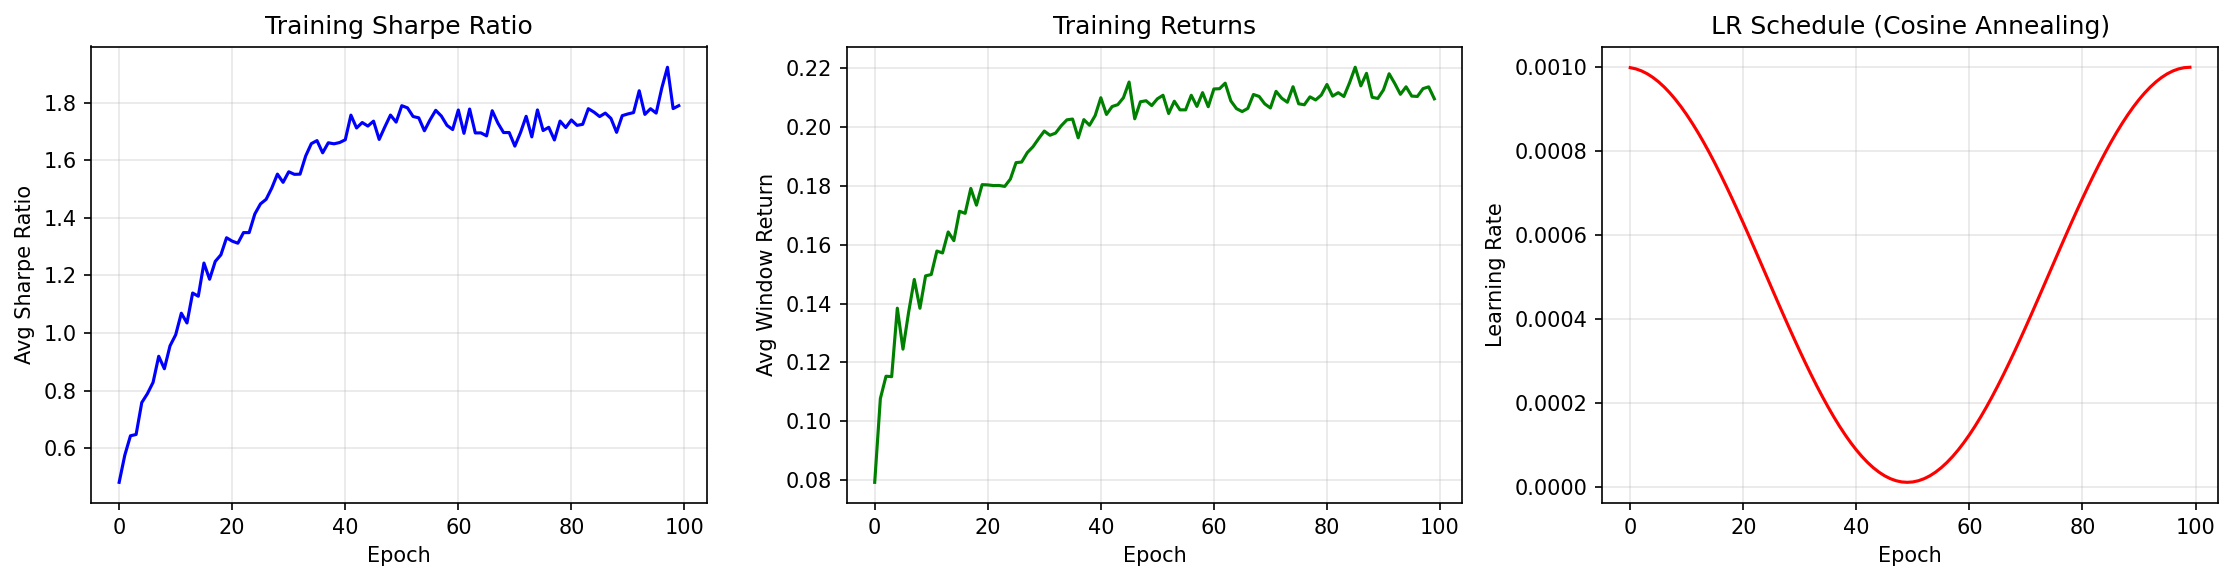
\includegraphics[width=\textwidth]{assets/training_curves.png}
  \end{center}
\end{frame}

\section{Results and Diagnostics}
\begin{frame}{Test Performance (24-Month Holdout)}
  \begin{table}
    \centering
    \begin{tabular}{lc}
      \toprule
      Metric & Value \\
      \midrule
      Monthly Sharpe & 0.1863 \\
      Annualized Sharpe & 0.6454 \\
      Total Return & 3.11\% \\
      Final Equity (\$1 base) & 1.0310 \\
      Annualized Return & 1.54\% \\
      Max Drawdown & 2.65\% \\
      \bottomrule
    \end{tabular}
  \end{table}
\end{frame}

\begin{frame}{Equity Curve and Drawdown}
  \begin{center}
    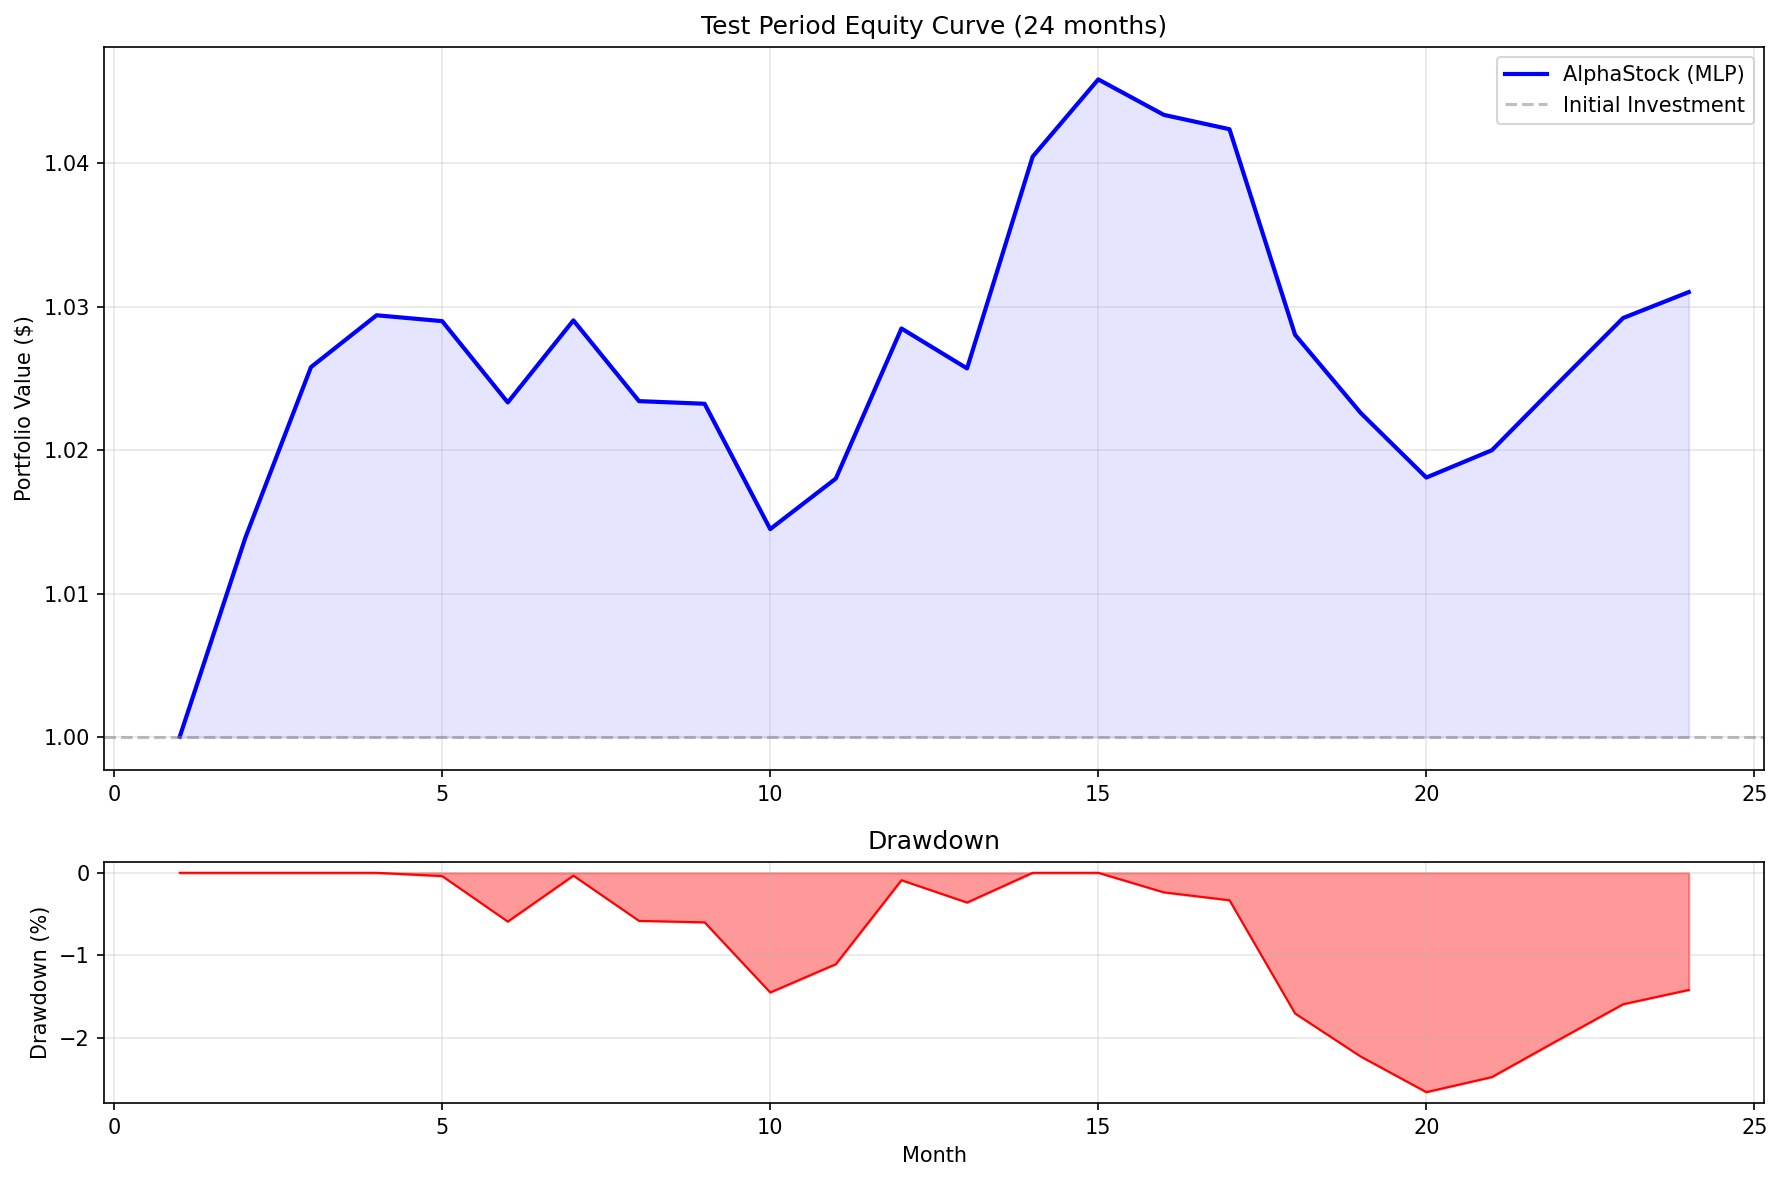
\includegraphics[width=\textwidth]{assets/equity_curve.png}
  \end{center}
\end{frame}

\begin{frame}{Return Distribution}
  \begin{center}
    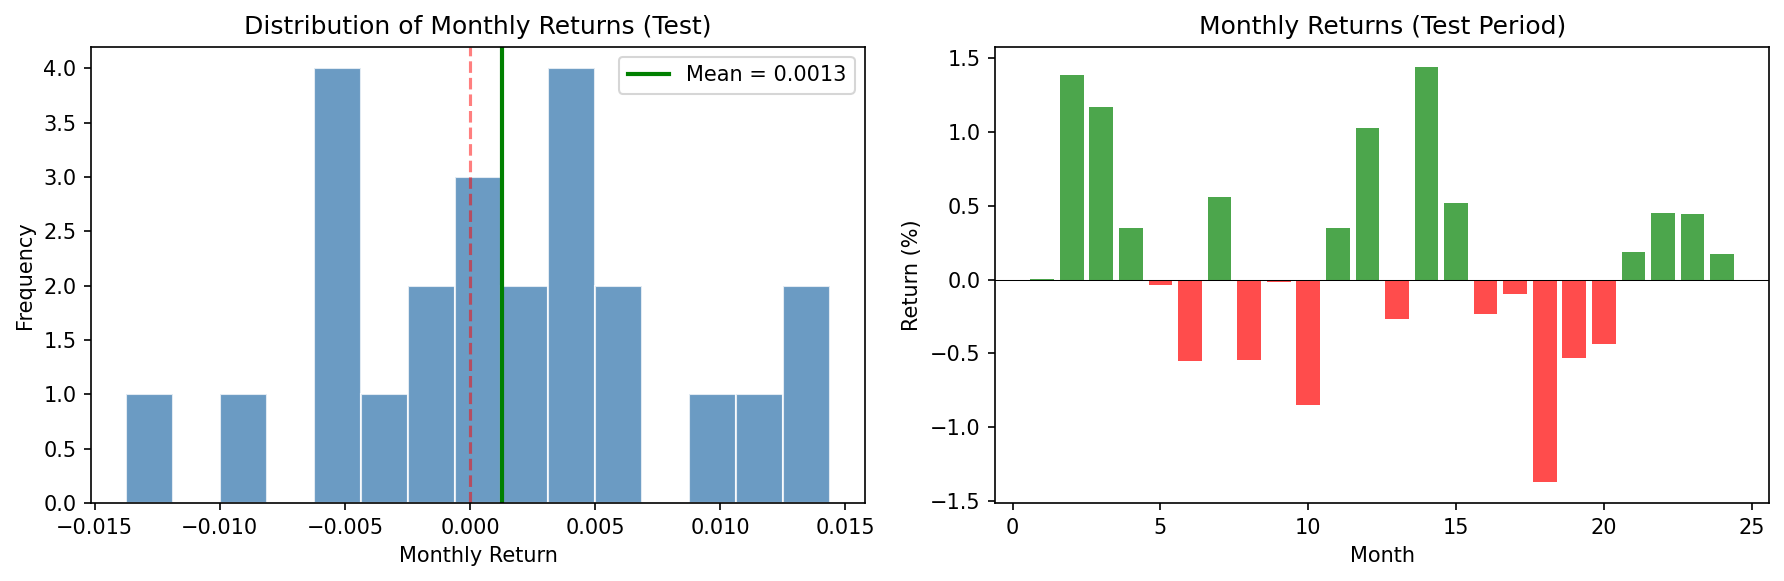
\includegraphics[width=\textwidth]{assets/returns_distribution.png}
  \end{center}
\end{frame}

\begin{frame}{Sharpe Gradient Weight Diagnostics}
  \begin{center}
    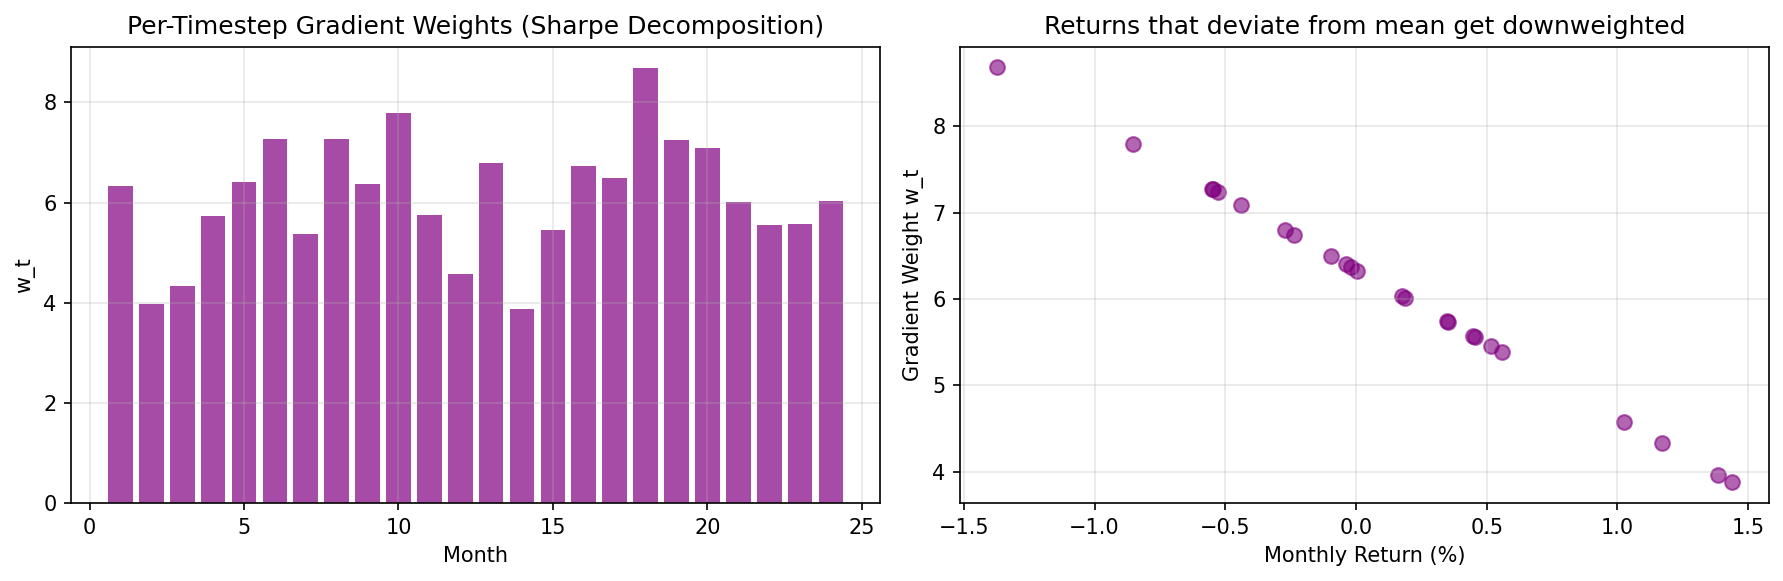
\includegraphics[width=\textwidth]{assets/sharpe_gradient_weights.png}
  \end{center}
\end{frame}

\section{Takeaways}
\begin{frame}{What This Project Demonstrates}
  \begin{itemize}
    \item Smooth continuation of the original AlphaStock proposal into a full Indian-market implementation.
    \item Practical model variant (MLP encoder) can preserve core AlphaStock logic with lower parameter complexity.
    \item Risk-aware training objective yields controlled drawdown with positive holdout performance.
    \item Codebase is reusable for future extensions: actor-critic, transaction costs, regime-aware features.
  \end{itemize}
\end{frame}

\begin{frame}{Next Steps}
  \begin{itemize}
    \item I am not fully satisfied with the current results, but I loved this project and will keep improving it through the summer.
    \item Add explicit benchmark comparison (e.g., index and equal-weight long-short).
    \item Include transaction cost and turnover penalties.
    \item Run multi-seed backtests and confidence intervals.
    \item Expand to multi-horizon training windows and stress periods.
  \end{itemize}
\end{frame}

\begin{frame}
  \centering
  {\Huge Thank You}
\end{frame}

\end{document}
